\chapter{\IfLanguageName{dutch}{Bijlagen}{Attachments}}{\label{ch:Bijlagen}}
\section{Verbinden met Cosmos DB via Gremlin API}
\begin{listing} [H]
    \begin{minted}{javascript}
         const Gremlin = require('gremlin');
         const config = require('../config/config');

         let client;

         function getClient() {
              if (!client) {
                   const authenticator = new Gremlin.driver.auth.PlainTextSaslAuthenticator(
                        `/dbs/${config.database}/colls/${config.collection}`, config.primaryKey
                   );
                   client = new Gremlin.driver.Client(
                        config.endpoint,
                        {
                             authenticator,
                             traversalsource: 'g',
                             rejectUnauthorized: true,
                             mimeType: 'application/vnd.gremlin-v2.0+json'
                        }
                   );
              }
              return client;
         }

         module.exports = { getClient };
    \end{minted}
    \caption[Voorbeeld verbinding met CosmosDB via Gremlin API.]{\label{fig:gremlinClient}Voorbeeld van hoe we verbinding maken met CosmosDB via Gremlin API.}
\end{listing}

\section{Voorbeeld Docker-compose bestand}
\begin{listing}[H]
    \begin{minted}{yaml}
        version: '3.8'
         services:
         elasticsearch:
              image: docker.elastic.co/elasticsearch/elasticsearch:8.13.4
              container_name: elasticsearch
              environment:
                   - discovery.type=single-node
                   - ES_JAVA_OPTS=-Xms512m -Xmx512m
                   - xpack.security.enabled=false
                   - network.host=0.0.0.0
              
              
              volumes:
                   - es_data:/usr/share/elasticsearch/data

         chatbot:
              build:
                   context: ../..
                   dockerfile: scripts/docker/Dockerfile.chatbot
              container_name: chatbot
              command: ["node", "scripts/chatbotPy.js"]
              volumes:
                   - ../..:/app
              depends_on:
                   - elasticsearch
              ports:
                   - "3000:3000"

         ollama:
              container_name: ollama
              image: ollama/ollama:latest
              
              volumes:
              - ollama_models:/root/.ollama
              restart: unless-stopped
              environment:
              - OLLAMA_HOST=0.0.0.0

         volumes:
              es_data:
                   driver: local
              ollama_models:
    \end{minted}
    \caption[Voorbeeld Docker-compose]{\label{fig:Docker-compose}Voorbeeld van een Docker-compose bestand.}
\end{listing}

\section{Voorbeeld Dockerfile voor NodeJS en Python}
\begin{listing}[H]
    \begin{minted}{dockerfile}
         # Basis image
         # We gebruiken hier NodeJS versie 20
         FROM node:20

         # Bepalen van de werkdirectory (waar alle bestanden komen)
         WORKDIR /app

         # installeren van NodeJS packages
         COPY package*.json ./
         RUN npm install

         # Kopieer de requirements.txt naar de container
         # Dit is een tekstbestand met de Python packages die we nodig hebben
         COPY requirements.txt ./

         # Kopieer alle bestanden naar de container
         COPY . .

         # Commando om Python te installeren
         RUN apt-get update && apt-get install -y python3 python3-pip

         # Dependencies installeren die nodig zijn voor de chatbot
         RUN pip3 install --no-cache-dir -r requirements.txt

         # Starten van de Node.js applicatie
         CMD ["node", "scripts/chatbotPy.js"]
    \end{minted}
    \caption[Voorbeeld Dockerfile]{\label{fig:dockerfile}Voorbeeld van een Dockerfile.}
\end{listing}

\section{Screenshot van de demo video}
\begin{figure}[H]
    \centering
    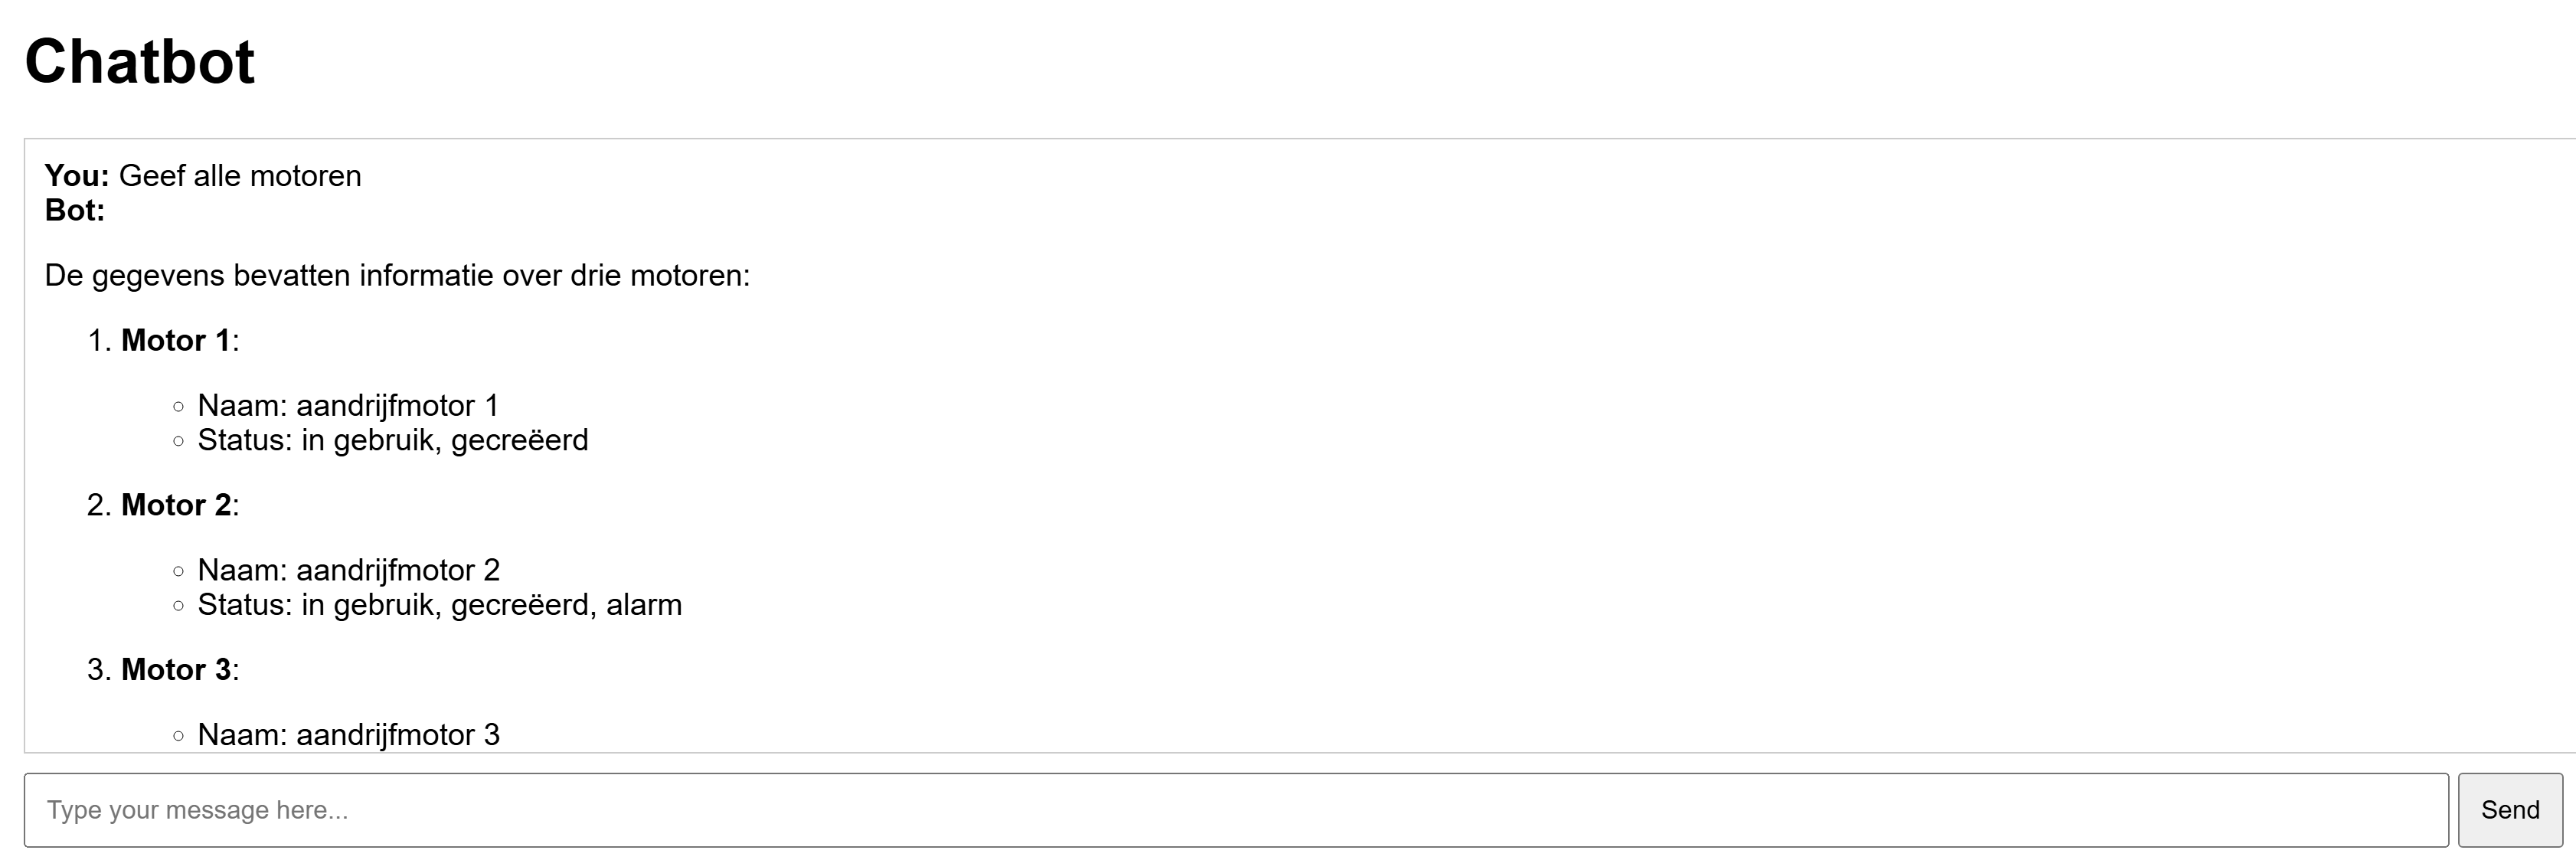
\includegraphics[width=0.8\textwidth]{./img/chatbot_response.png}
    \caption[Demo video (screenshot)]{\label{fig:demo}Screenshot van de demo video.}
\end{figure}

\section{Workflow van de chatbot}
\begin{figure}[H]
    \centering
    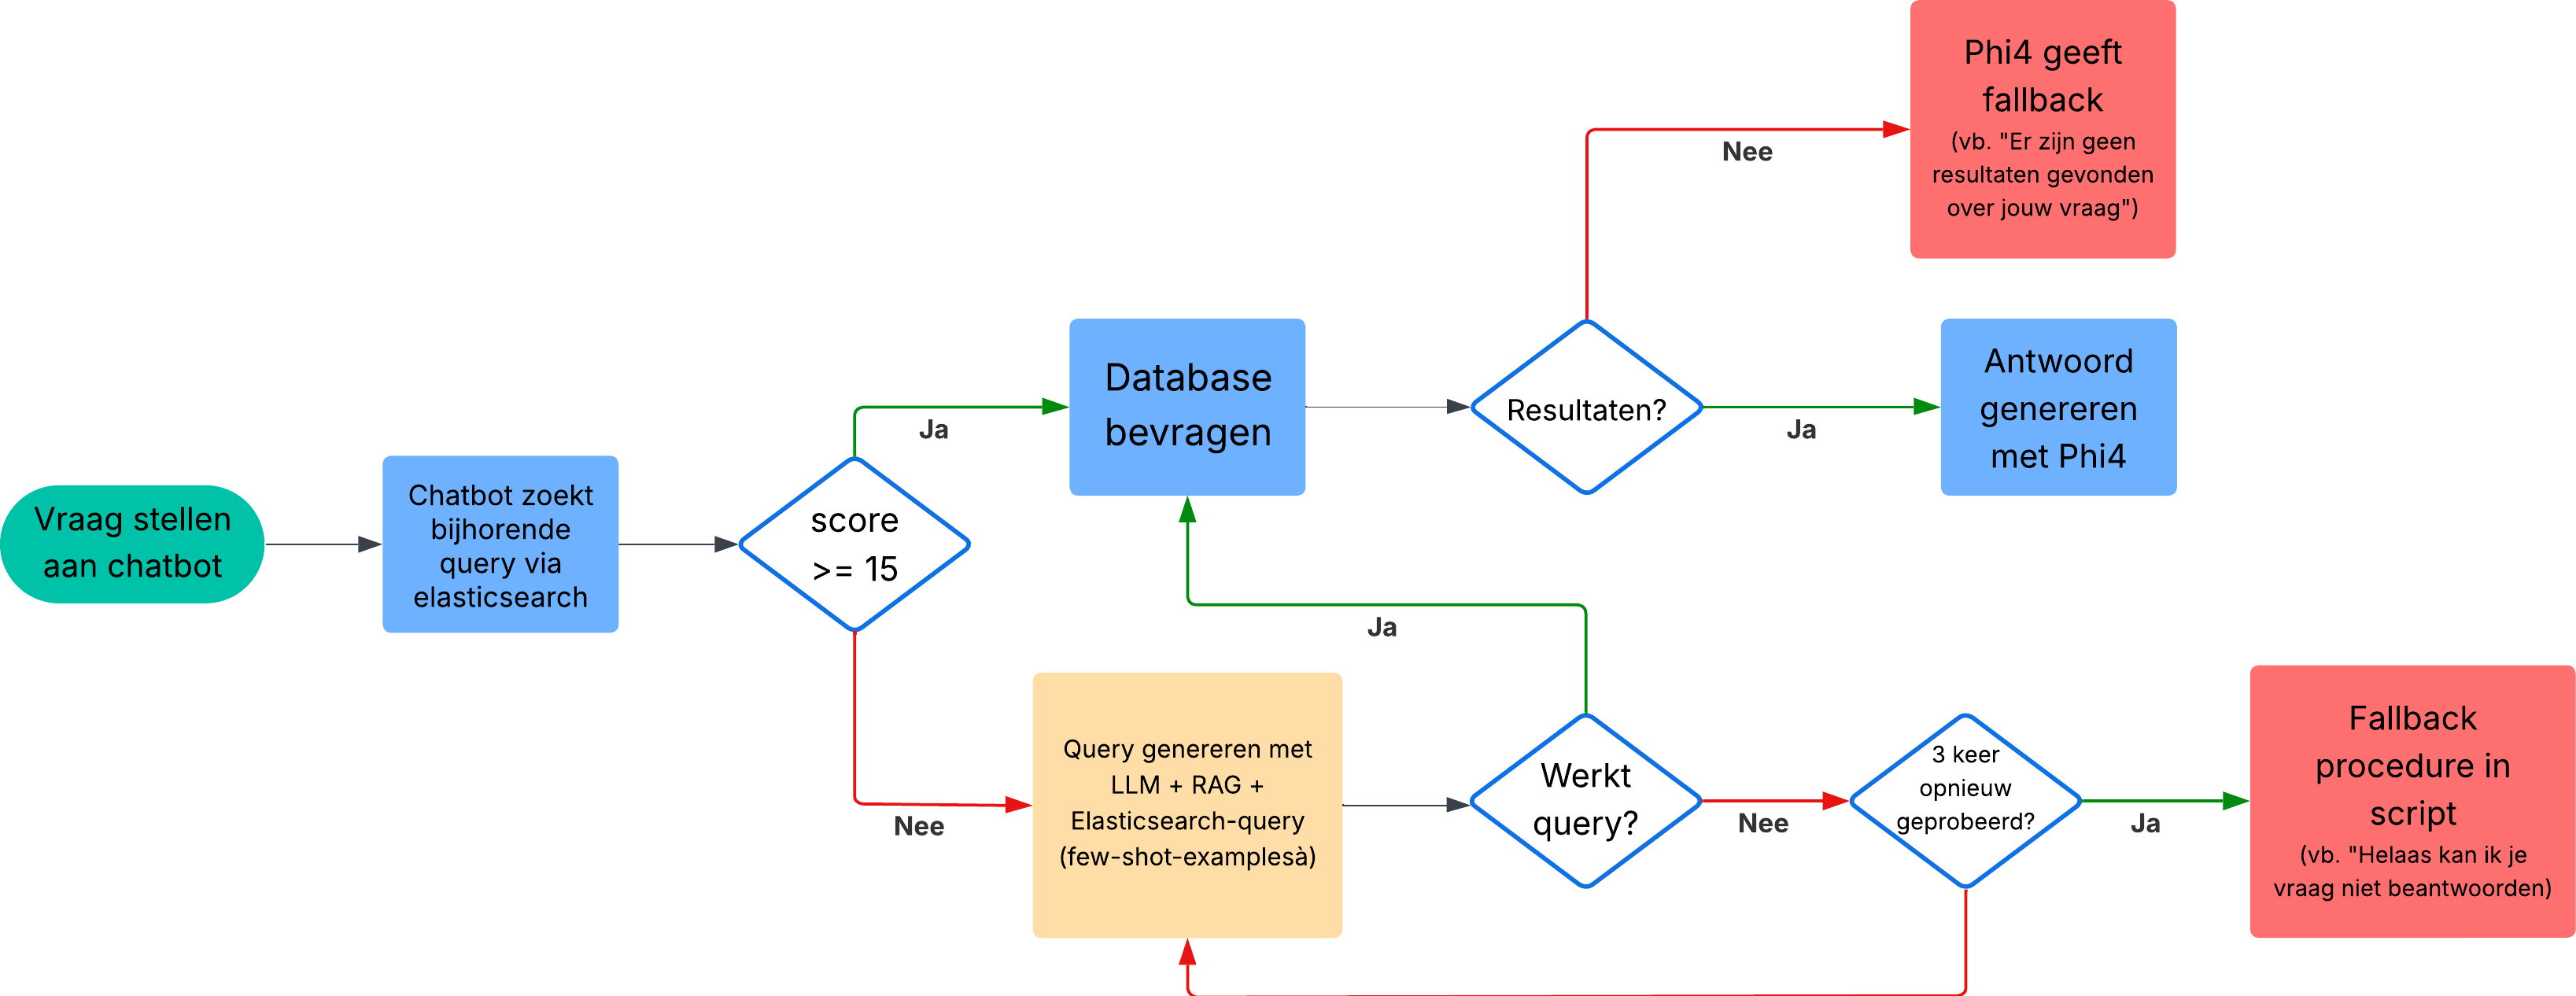
\includegraphics[width=0.8\textwidth]{./img/chatbot_workflow.png}
    \caption[Workflow van de chatbot]{\label{fig:chatbot_workflow}Workflow van de chatbot, van vraag tot antwoord.}
\end{figure}

% \section{Voorbeeld Elasticsearch query bepalen}
% \begin{listing}[H]
%     \begin{minted}{javascript}
%          if response["hits"]["hits"]:
%             best_hit = response["hits"]["hits"][0]
%             score = best_hit["_score"]
%             if score >= 12:
%                 query = best_hit["_source"]["antwoord"]
%                 logging.debug(f"Vraag gevonden in Elasticsearch met score {score}: {query}")
%                 logging.debug(f"Vraag: {question} - Query: {query}")
%                 return query
%             else:
%                 logging.debug(f"Vraag gevonden in Elasticsearch, maar score ({score}) is te laag.")
%                 previous_query = best_hit["_source"]["antwoord"]  # Sla de vorige query op
%                 if previous_query:
%                     query = generate_query_from_llm(question, context, previous_query, error)
%                     return query
%     \end{minted}
%     \caption[Voorbeeld Elasticsearch query bepalen]{\label{fig:elasticsearchQuery}Voorbeeld van hoe we een Elasticsearch query bepalen.}
% \end{listing}